\section{Active Fluid Model Fitting of Cortical Flow Measurement in \textit{C. elegans} embryos}

To ascertain the manner in which active stress and effective viscosity depend upon
actin and myosin densities, I studied cortical flow in the \textit{C. elegans}
single cell embryo during polarity maintenance phase. The single cell \textit{C. elegans}
embryo poses a viable model system wherein to determine how active stress and
effective viscosity depend on constitutive properties of the cytoskeleton. During
the \textit{C. elegans} first division cycle, cell fate determinants and small regulatory
GTPases are segregated between distinct anterior and posterior domains, and these 
asymmetries are actively sustained through regulatory feedback for ~5 minutes 
during the polarity maintenance phase. [11] As displayed in Fig. \ref{fig:measure_flow} this system is 
characterized by a spatially varying distribution of myosin motors 
in the presence of persistent unidirectional cortical flow from the posterior pole 
towards a band of cytoskeletal aggregation near the midline.

In addition to the steady state velocity profile, the \textit{C. elegans} embryo provide a number of
advantages that made these measurements easier. The events of polarization are highly
stereotyped and reproducible, allowing for comparison between experiments. Transgenic strains
expressing fluorescently-tagged variants of myosin-II and F-actin binding proteins (e.g. utrophin and
moesin), allowing for simultaneous visualization of F-actin and myosin by fluorescence microscopy.
In addition, the superficial cortical layer allows for high quality microscopy necessary for the
experiments, and the cell geometry allows simplification to a 2D system. Finally, an important factor
necessary for constraining the theory is a fine level of control over the densities of both actin and
myosin, which can be supplied in the C. elegans embryo by RNAi depletion of nearly any gene
expressed in the germline. [12]



\subsection{Obtaining spatially resolved simultaneous measurement of actin and myosin densities.}

Rationale: Actin and myosin are assumed to be the drivers of cortical flow and their density profiles
and gradients are therefore important variables necessary to parametrize the functions of active stress
and effective viscosity upon which the theory is based.

To obtain the density profile, I used interleaved HILO microscopy timelapses to obtain
simultaneous images of myosin and actin in the C. elegans embryo during the single celled polarity
maintenance phase. Next, I coarse grained the image using image processing blurs or a fixed square
bin so that microscopic inhomogeneity is removed from the measurement. Limiting the analysis to one
dimension improved the measurement quality and made the mathematics simpler so an average
density taken along cross section lines running perpendicular to the embryo AP axis was computed.
The example in Fig. \ref{fig:measure_flow} displays a typical fluorescence image of the myosin localization in the embryo
along with the AP projection axis. The myosin fluorescence profile changes gradually
over the course of five minutes with a period of particular stability lasting roughly two minutes.





\subsection{Obtaining spatially resolved measurement of cortical flow velocities.}
To obtain a flow profile, I analyzed the myosin interframe displacements with
particle image velocimetry (PIV). I averaged a set of contiguous frames from the videos prior to blurring or binning in order to obtain a more clear image and provide a larger flow
displacement between PIV analyzed frames. The PIV algorithm is assumed to maintain a nearly
constant absolute margin of error so maximizing interframe flow distance while still maintaining
consistent results minimizes relative error. I selected a region of interest that remained
consistent throughout all experiments and encompassed the entirety of the dilating and contracting
regions.

The PIV algorithm was an FFT multipass with window deformation and a postprocessing
clean up that rejects and interpolates any velocity with a speed greater than ~3 times the standard
deviation.[13] Only the on axis motion is relevant at this time so the output velocity vectors will be
projected onto a line parallel to the AP axis. This component of the flow velocity was averaged
along the cross sections running perpendicular to the AP axis as before. The diagram below illustrates
a typical PIV flow analysis on the left. On the right, the projection of the flow velocity onto the AP
axis is shown to vary slowly in magnitude over the course of 5 minutes and to maintain the same
overall shape.




\subsection{Using the data to constrain a basic active fluid model}
I compared these measurements to the theoretical predictions by setting up a few nonlinear
functional fits of the velocity, effective viscosity and active stress as a function of myosin
density using a nonlinear least-squares fitting solver with the equation

\begin{equation}
v(x) = C_1 e^{x/l}+C_2 e^{-x/l}+ \int_{a}^{b} \frac{\delta\mu}{\delta x}(e^{(x'-x)/l}+e^{(x-x')/l}
\end{equation}

where $l$ is a length scale of force falloff and the constants $C_1$, $C_2$ are constrained by the boundary conditions at the points $a$ and $b$ in the embryo, $v(a) = v_a$ and $v(b)=v_b$.  See [Bois et al] for more details on this equations derivation.

Data fitting was carried out in MATLAB by passing a starting guess for the fitting coefficients to lsqnonlin along with the function defined above. 


\begin{figure}[h!]
	\centering
	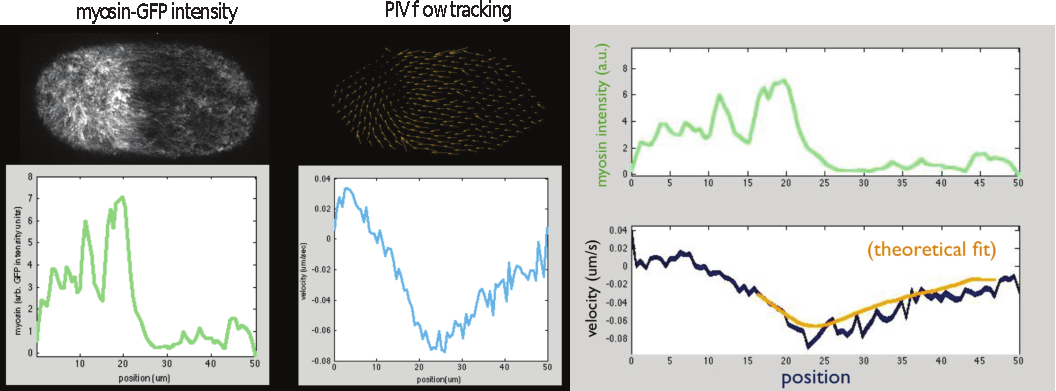
\includegraphics[width=\hsize]{data/prelim_flow.pdf}
	\caption{\label{fig:measure_flow}  Measurement of myosin intensity and flow profile.  These measurements fit a theoretical model of active fluid flow.  }
\end{figure}

The results of this analysis showed that, indeed, an active fluid function akin to that used in [Mayer and Grill] is capable of explaining the observed flow profiles in \textit{C. elegans} embryos.  


\subsection{Disruption of Flow by Myosin Depletion}

The above experiment only sampled a limited region of myosin-actin state space if only analyzed in wild type.
Using only data from this limited region does not uniquely determine the form of the
functions that satisfy the equations of motion. I needed to test outside this range by varying the
concentration of actin and myosin independently in order to adequately constrain the fitted equations
of active stress and effective viscosity.

RNAi depletion is a common practice used to decrease the cellular concentration of endogenously
expressed proteins in C. elegans. By feeding ssRNA containing \textit{E. coli} to mother nematodes, the
mRNA in the nematode germline is progressively silenced and the remaining protein decays away. I used this technique to lower the expression of myosin regulatory light chain kinase (MRCK), which is an upstream regulator of myosin.
Overall
myosin density decreases with a depletion of MRCK.
We assume that the degree of
depletion can be assessed by integrating the myosin density profile over the length of the cell.

Gene depleted embryos were imaged and processed in the exact same
manner as described above for wild type.

\begin{figure}[h!]
	\centering
	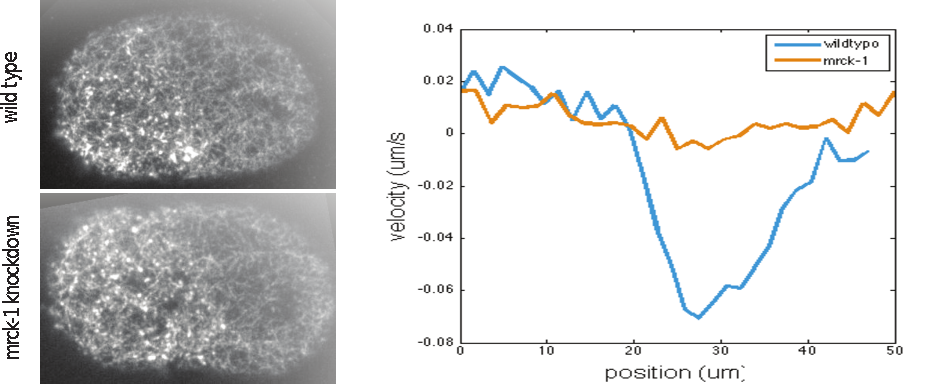
\includegraphics[width=\hsize]{data/flow_mrck_kd.pdf}
	\caption{\label{fig:measure_flow_nomyo}  Measurement of actin distributions and flow profiles for mrck-1 knockdown embryos.  MRCK-1 is an upstream regulator of myosin.  }
\end{figure}

As shown in Fig. \ref{fig:measure_flow_nomyo}, the actin densities were largely unaffected.  Nevertheless, the myosin density (not shown) and flow profile (Fig. \ref{fig:measure_flow_nomyo}, right) were reduced.  Progressive depletion of MRCK also showed a graded response to myosin depletion, indicating that myosin activity imparts internal force in a dose dependent manner.

\section{Stabilization of Filament Turnover with Jasplakinolide Treatment}

Jasplakinolide is a small molecule inhibitor of actin depolymerization.  When treated with jasplakinolide, actin filaments can be stabilized to have very long filament lifetimes.  To study the effect of filament stabilization on cortical flows, Jon Michaux treated embryos with jasplakinolide and imaged the actin cytoskeleton with utrophin::GFP.  The results were striking, and clearly showed that loss of turnover resulted in distrupted flows.  Moreover, in some cases, the treatment didn't just result in a stalling of flows, but also led to a tearing of the cortex followed by further transient contraction.  Nevertheless, all embryos with jasplakinolide treatment eventually stalled and failed to continue with normal polarization and division.

\begin{figure}[h!]
	\centering
	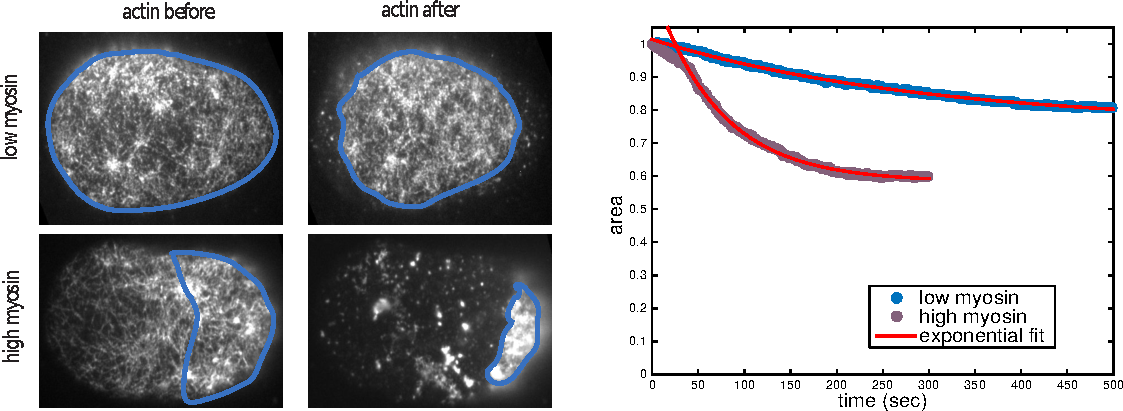
\includegraphics[width=\hsize]{data/jasp_flow_stop.pdf}
	\caption{\label{fig:jasp_flow_stop}    }
\end{figure}

I made an attempt to quantify the degree of contraction possible in jasplakinolide treated embryos using hand tracking of fiducial markers in Jon's videos.  As can be seen in Fig. \ref{fig:jasp_flow_stop}, whether the cortex stalled or tore, the resulting strain asymptotically approached some limiting strain.  This is in sharp contrast to the persistent strains ($\gamma>1$) possible in the steady state flows found when turnover is present.